\chapter{Arhitecturi de conectare  MPTCP prin proxy}
\label{sec:arch_upb}

MPTCP RFC\cite{rfc6824bis}, \cite{mptcp-nsdi} este un upgrade la TCP
care permite conectarea simultană prin interfețe multiple, fără a
recompila aplicațiile. O aplicație folosește în continuare API-ul de
BSD sockets, dar beneficiază de conexiunile multiple disponibile în
telefoanele de astăzi: WiFi, 4G, si Bluettoth. Pentru a beneficia de
funcționalitatea MPTCP, atât serverul cât si clientul trebuie
modificate. Deoarece multe servere nu implementează încă MPTCP,
soluția temporara este de a ruta tot traficul MPTCP printr-un proxy
care continuă conexiunea cu TCP clasic până la serverele legacy.


\section{Protocoale din familia SOCKS}

\subsection{SOCKS 5}

Protocolul SOCKS este folosit pentru a crea conexiuni TCP către destinații arbitrare folosind un proxy.
În ultima versiune standardizată a protocolului (versiunea 5), durează doua RTT-uri (sau 3, dacă se face și autentificare) până când datele pot circula între client și server.

\begin{figure}[h]
	\centering
	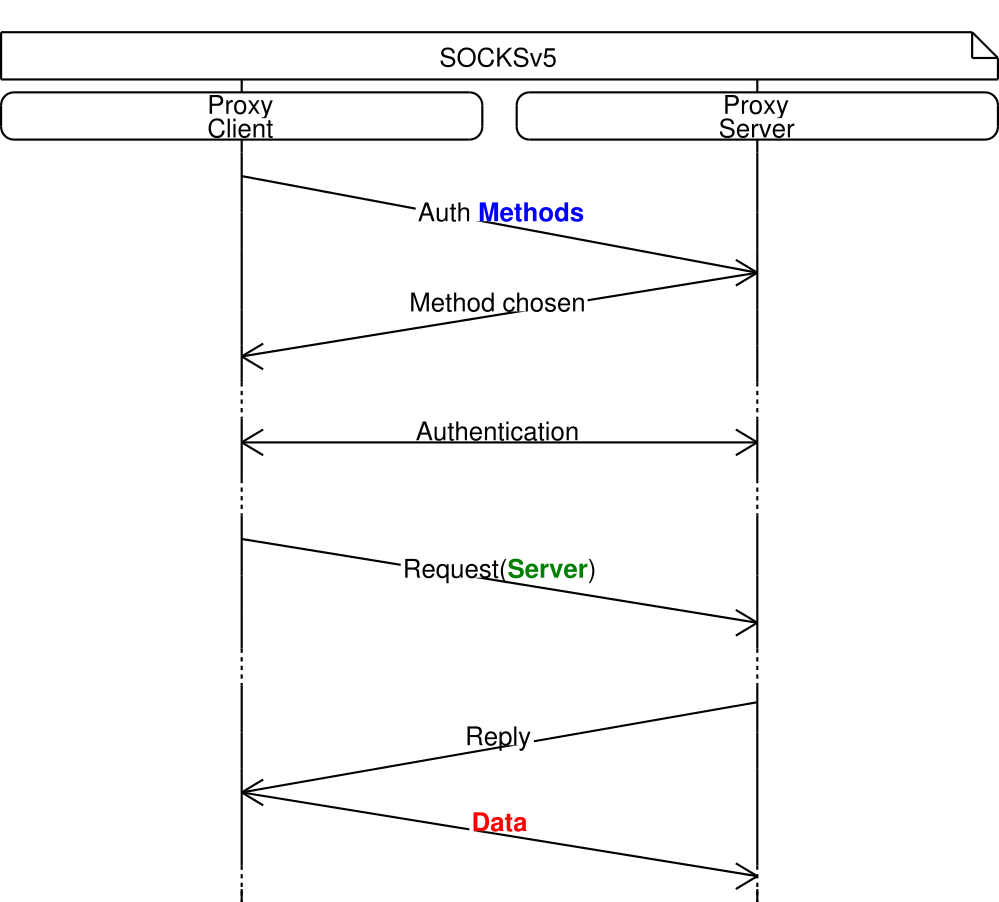
\includegraphics[scale=0.7]{figures/socks/socks5op.png}
	\caption{Mod de operare SOCKS 5}
    	\label{fig:socks5op}
\end{figure}

In SOCKS 5 (versiunea curentă a protocolului, v. fig \ref{fig:socks5op}), clientul deschide o conexiune căte proxy si parcurge urmatoarele etape înainte să transmită date către server:
\begin{itemize}
	\item Negocierea metodei de autentificare (1 RTT): Clientul trimite un mesaj care conține metodele de autentificare suportate. Proxy-ul răspunde cu metoda de autentificare aleasă.
	\item Autentificarea propriu-zisă (0-1 RTT-uri): Acest pas poate să lipsească, dacă nu se face autentificare. Altfel, durează tipic un RTT.
	\item Crearea socket-ului (1 RTT): Clientul trimite adresa și portul server-ului la care vrea sa se conecteze. Proxy-ul încearcă să onoreze cererea clientului și îi trimite un răspuns cu rezultatul.
\end{itemize}


\subsection{SOCKS 6}

Am dezvoltat versiunea 6 a protocolului SOCKS, pe care o propunem pentru standardizare în cadrul IETF. Momentan se află in starea de Internet Draft~\cite{socks6}.
Principalele îmbunătățiri introduse în această versiune sunt:
\begin{itemize}
	\item Clientul are un comportament optimist și trimite cât mai multe informații către proxy, fără a aștepta să se termine autentificarea.
	\item Semanticile cererilor imită semanticile TCP Fast Open~\cite{rfc7413}. În cerere, clientul poate include și potențialul payload pentru SYN-ul inițial trimis către server.
	\item Protocolul poate fi extins folosind opțiuni, similare cu opțiunile TCP.
	\item Folosint opțiunile menționate mai sus, se pot implementa scheme de autentificare în 0 RTT-uri.
\end{itemize}


\begin{figure}[h]
	\centering
	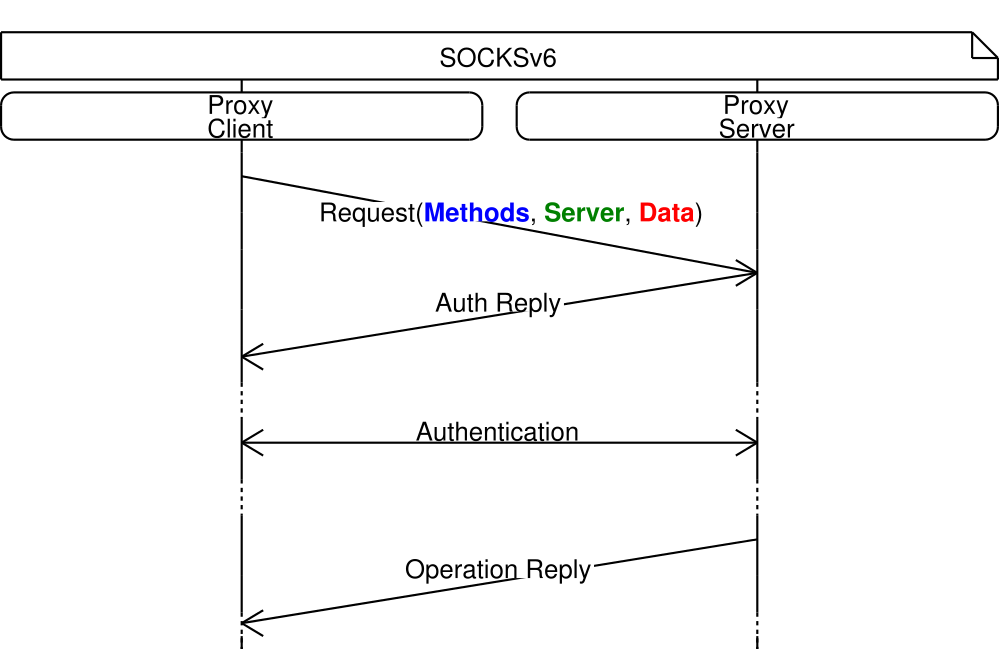
\includegraphics[scale=0.7]{figures/socks/socks6op1st.png}
	\caption{Mod de operare SOCKS 6 (prima conexiune cu autentificare)}
    	\label{fig:socks6op1st}
\end{figure}

\begin{figure}[h]
	\centering
	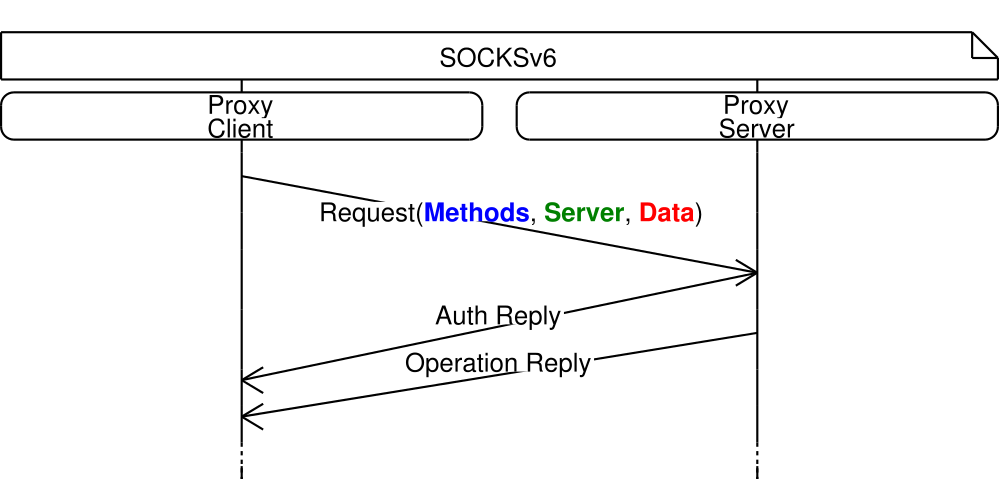
\includegraphics[scale=0.7]{figures/socks/socks6op2nd.png}
	\caption{Mod de operare SOCKS 6 (conexiuni ulterioare)}
    	\label{fig:socks6op2nd}
\end{figure}

Atunci când un client SOCKS 6 încearcă să se conecteze la un server, deschide o conexiune către un proxy (v. fig. \ref{fig:socks6op1st}) .
Clientul începe prin a trimite o cerere (SOCKS Request), care conține, printre altele:
\begin{itemize}
	\item Metodele de autentificare cunoscute de client.
	\item Adresa și portul server-ului.
	\item Primii octeți din fluxul de date destinat server-ului.
\end{itemize}

Proxy-ul răspunde cu un Authentication reply, care indică protocolul de autentificare care trebuie folosit.
Apoi se execută protocolul de autentificare ales, lucru care poate dura un RTT sau mai mult.

Dacă autentificarea s-a terminat cu succes, proxy-ul încearcă să creeze conexiunea cerută de client, si trimite un Operation Reply, care indică dacă s-a putut realiza conexiunea sau nu.

În cererile ulterioare, clientul poate să includă date de autentificare in cerere (Request), lucru care îl scutește de etapa de autentificare (fig. \ref{fig:socks6op1st}).
Astfel, se poate obține un răspuns de la server intr-un singur RTT, cu 2-3 RTT-uri mai rapid decât cu SOCKS 5.



\chapter{Folosirea MPTCP în sistemul de operare Android}
\label{sec:mptcp_android}
\section{Imaginea Android}

În acest proiect s-au folosit dispozitive mobile Samsung Galaxy S7 Edge. Acestea rulează în mod implicit o imagine a sistemului de operare Android de la Samsung, care include implementarea protocolului MPTCP în kernel. 

Imaginea de Android (stock ROM) folosită este identificată prin urmatoarele:
\begin{enumerate}
	\item Model number: SM-G935F
	\item Baseband version: G935FXXU1DQA3
	\item Build number: NRD90M.G935FXXU1DQAS
	\item Android version: 7.0
\end{enumerate}

Imaginea de Android stock este rescrisă folosind utilitarul Odin, în timp ce dispozitivul este în modul \texttt{Download}. Astfel, se vor rescrie partițiile boot, system și recovery ale dispozitivului. Prin această metodă, telefonul este adus înapoi la starea inițială, în cazul întâlnirii unei erori pe parcursul root-ării dispozitivului. 

\section{Rootarea dispozitivului mobil}

Pentru activarea și configurarea protocolului MPTCP este nevoie de un telefon rootat deoarece comenzile necesare nu pot fi rulate decat din contul root (sysctl, ip rule, ip route).

Pentru root-area dispozitivului este nevoie de utilitarele Odin, TWRP și SuperSU. Se foloseste imaginea de recovery TWRP pentru modelul \emph{hero2lte}. Se scrie această imagine folosind Odin, în timp ce telefonul este în modul \texttt{Download}. Astfel, se va rescrie partiția de recovery a dispozitivului. 

Apoi se intră în modul \texttt{Recovery} al telefonului pentru a accesa meniul aplicației TWRP. Se formatează partiția de date și se instalează aplicația SuperSU care rootează telefonul. 

În final se boot-ează telefonul în modul normal si se instalează aplicația Android TWRP. Apoi, în adb shell se poate introduce comanda \texttt{su} pentru a intra în contul utilizatorului root. Se testează daca se poate activa protocolul MPTCP folosind utilitarul \texttt{sysctl}.

Din cauza formatării partiției de date, este posibil ca utilitarul \texttt{adb} sa dea mesajul "unauthorized device" și să nu putem obține un shell pe dispozitiv. Acest lucru se poate rezolva prin boot-area în modul Recovery în TWRP, și copierea cheii publice asociată utilitarului \texttt{adb} pe dispozitiv. După aceea, se va porni sistemul de operare Android și utilizatorul se poate conecta la telefon folosind \texttt{adb shell}.

\section{Configurarea protocolului MPTCP}

Configurarea protocolului MPTCP se face prin următorii pași:
\begin{enumerate}
	\item Se activează WiFi și LTE în Settings
	\item Se activează opțiunea Settings $->$ Developer Options $->$ Mobile Data Always Active
	\item Se activează protocolul MPTCP folosind utilitarul \texttt{sysctl}
	\item Se crează câte un tabel de rutare diferit pentru fiecare interfață, care vor fi folosite pentru rutarea pe baza adresei sursă, prin comanda \texttt{ip rule}
	\item Se configurează cele două tabele de rutare prin adăugarea unei rute default, folosind gateway-ul fiecărei conexiuni, prin comanda \texttt{ip route} 
	\item Se adaugă o rută default globală pentru traficul normal în Internet, folosind gateway-ul uneia din cele două conexiuni, prin comanda \texttt{ip route}
\end{enumerate}
Pașii 3-6 se pot automatiza sub forma unui script bash, care se poate rula după boot-area dispozitivului sau la cererea utilizatorului, atunci când dorește activarea MPTCP.  Se va crea și configura cate un tabel de rutare pentru fiecare interfață activă (cu adresă IP).

Scriptul folosește binarul \texttt{awk}. Acesta este obținut prin instalarea aplicației BusyBox și folosirea ei pentru a instala binarele puse la dispoziție.

De asemenea, la dezactivarea unei interfețe sau la pierderea conexiunii pe o interfață, trebuie șteasă tabela de rutare asociată cu acea interfață, prin comanda \texttt{ip rule}. 

\section{Aplicația de monitorizare a conexiunilor de rețea}

A fost dezvoltată o aplicație Android, numită ConnectivityMonitor,  care monitorizează starea conexiunilor WiFi și LTE, și reconfigurează tabelele de rutare pentru MPTCP atunci cand se modifică starea unei conexiuni. De asemenea, poate fi folosită pentru vizualizarea statisticilor colectate sau pentru rularea scripturilor/executabilelor. 

Funcționalitatea de bază a aplicației este de a activa și configura MPTCP pentru folosirea celor două interfețe de rețea (WiFi și LTE). Utilizatorul poate activa si dezactiva MPTCP folosind o opțiune din fereastra de setări. În spate, aplicația rulează scripturi bash în mod privilegiat (folosind utilitarul \texttt{su}).

Aplicația este implementată să primească notificări atunci când se schimbă starea unei interfețe de rețea (conectare și deconectare). In cazul unui eveniment de conectare, se crează și populează tabela de rutare asociată interfeței. În cazul unui eveniment de deconectare, se șterge tabela de rutare asociată acelei interfețe.

ConnectivityMonitor colectează informații despre cele doua interfețe, periodic, o data la 30 secunde. Pentru interfața de WiFi se colectează: numărul de bytes trimiși și primiți, RSSI, RTT, MCS și frecvența. Pentru interfața de LTE se colectează: numărul de bytes trimiși și primiți, RSSI, CID, TAC. De asemenea, este salvat periodic nivelul bateriei. 

Tot din aplicație se pot rula scripturi bash, Python sau executabile, pentru evaluarea experimentală a caracteristicilor traficului de rețea (lățime de bandă, lantență, etc.).

Evenimentele de conectare/deconectare a interfețelor de rețea, datele colectate și rezultatele scripturilor sunt salvate in baza de date, care este salvată periodic în cloud, în spațiul de stocare oferit de Firebase, intr-un folder ce are ca nume IMEI-ul telefonului.

Informațiile din baza de date pot fi analizate și corelate pentru determinarea procentului de timp în care utilizatorul are acces la ambele interfețe de rețea, disponibilitatea lor atunci când utilizatorul dorește să le utilizeze, și perfomanța acestora în  acele momente.

\section{Testarea soluțiilor proxy}

De cele mai multe ori serverul cu care comunică dispozitivul mobil nu o să folosească protocolul MPTCP. De aceea avem nevoie de folosirea unui proxy, care va fi o stație intermediară cu IP public. Comunicația între dispozitivul mobil si proxy se face prin MPTCP iar între proxy si server se va folosi în general TCP. Dispozitivul mobil este conectat la WiFi și LTE, iar atunci când rulează protocolul MPTCP, va folosi ambele interfețe.

Soluțiile proxy testate în cadrul acestui proiect au fost: 1) Shadowsocks pe dispozitivul mobil și pe stația proxy, 2) ProxyDroid pe dispozitivul mobil și SS5 pe proxy. Toate componentele software folosite sunt open-source. În urma testelor preliminare, s-a constatat că soluția a doua (ProxyDroid și SS5) este cea  mai eficientă din punct de vedere al consumului de resurse pe sistemulul proxy, și folosește SOCKS v4 și v5, în timp ce Shadowsocks folosește un protocol custom.

Scenariile în care s-a facut evaluarea experimentală sunt: 1) comunicația directă între dispozitivul mobil și server folosind protocolul TCP, 2) comunicația directă folosind MPTCP, 3) comunicația prin proxy, folosind MPTCP între mobil și proxy, și TCP între proxy și server, ca în Figura \ref{fig:proxy}. 

\begin{figure}[h]
	\centering
	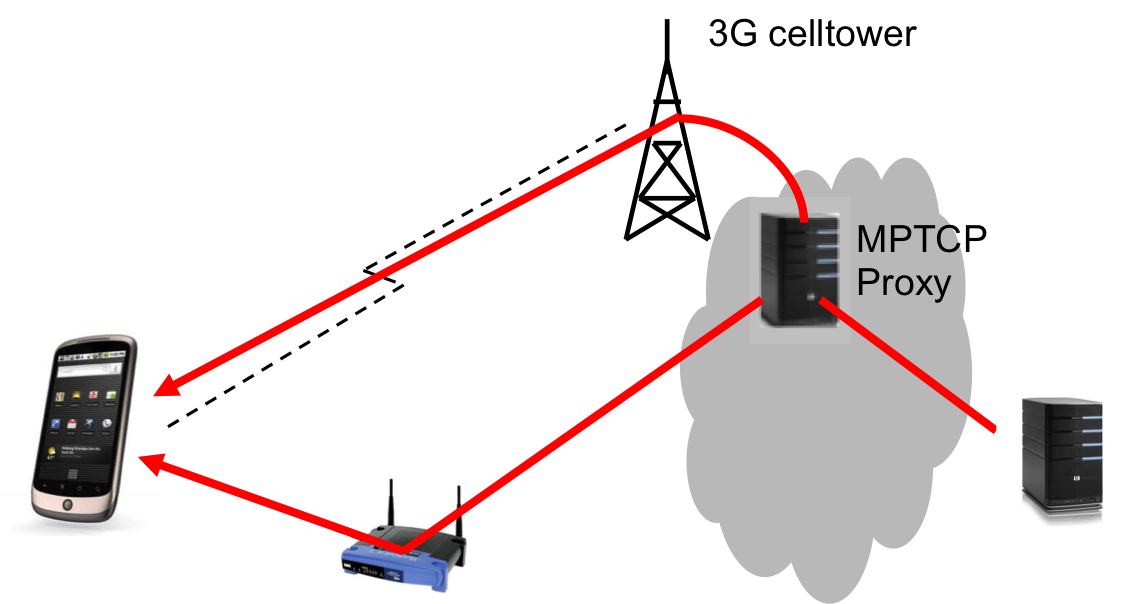
\includegraphics[scale=0.7]{figures/45g_proxy.png}
	\caption{Comunicația prin proxy}
    	\label{fig:proxy}
\end{figure}

Metricile folosite au fost round-trip time (RTT) și throughput. S-au folosit scripturi Python și utilitare open-source pentru măsurarea valorilor acestor metrici în scenariile considerate.

Tabelul \ref{tab:rtt} prezintă valorile RTT-ului în cele 3 scenarii. Pentru acest experiment s-a implementat un script Python care trimite date la un server si masoara timpul pana la primirea raspunsului. S-au trimis date de 1000 de ori si s-au calculat statistici pe baza timpului obținut la fiecare iterație (minim, maxim, media, mediana, deviația standard).

Se poate observa că nu există o diferență notabilă între comunicația directă cu TCP și cea cu MPTCP din punct de vedere al RTT-ului. Folosirea unui proxy introduce o latență de aproximativ 3ms, care este o valoare acceptabilă deoarece nu afectează calitatea experienței utilizatorului.

\begin{table}[h]
\centering
\caption{RTT}
\label{tab:rtt}
\begin{tabular}{l | c c}
\hline
& Interval RTT (ms)  & RTT median (ms) \\
\hline
Telefon --(TCP) --$>$ Server  & 3-9 &  7.08  \\
Telefon --(MPTCP) --$>$ Server  & 3-8  & 7.29 \\
Telefon --(MPTCP)--$>$ Proxy --(TCP)--$>$ Server & 5-11  & 10.28 \\
\hline
\end{tabular}
\end{table}

Tabelul \ref{tab:throughput} prezintă valorile throughput-ului în următoarele scenarii: 1) comunicația directă între o stație desktop (prin Ethernet) și server, fara proxy, 2) comunicația directă între o stație desktop (prin WiFi) și server, fara proxy, 2) comunicația directă între mobil (prin WiFi) și server, fără proxy, 3) comunicația între mobil (prin WiFi) și server, prin proxy.

\begin{table}[h]
\centering
\caption{Throughput}
\label{tab:throughput}
\begin{tabular}{l | p{1.5cm} p{1.5cm} p{1.5cm} p{1.5cm}}
\hline
& Uplink (average) & Uplink (max) & Downlink (average) & Downlink (max) \\
\hline
Stație (eth) --$>$ Server & 933 & 945 & 501 & 611 \\
Stație (wifi) --$>$ Server & 582  & 600  & 501  & 566  \\
Telefon (wifi) --$>$ Server & 497 & 516 & 533 & 562 \\
Telefon (wifi) --$>$ Proxy --$>$ Server & 233 & 287 & 317 & 413 \\
\hline
\end{tabular}
\end{table}

În urma rezultatelor obținute, se poate observa că folosirea interfeței WiFi în loc de Ethernet, reduce considerabil throughput-ul traficului de la client la server (uplink). De asemenea, observăm că  folosirea unui proxy reduce throughput-ul atât la uplink cât și la downlink.

\section{Planul de colectare și corelare al datelor}

Următorul pas este efectuarea unui experiment în care un număr de utilizatori vor folosi în mod normal telefoane, timp de 30 de zile, cu următoarele componente software:
\begin{itemize}
	\item Protocolul MPTCP activat
	\item Aplicația ConnectivityMonitor gestionează conexiunile de WiFi și LTE și configurează tabelele de rutare MPTCP
	\item Aplicația ProxyDroid trimite tot traficul către un sistem proxy ce rulează SS5 și are MTPCP activat 
\end{itemize}

Aplicația ConnectivityMonitor va colecta periodic date legate de starea conexiunilor WiFi și LTE. Tabelul \ref{tab:date} include tipurile de date care vor fi colectate în cadrul acestui experiment.

\begin{table}[h]
\centering
\caption{Tipuri de date colectate}
\label{tab:date}
\begin{tabular}{c | c}
\hline
Interfata & Tip de date  \\
\hline
WiFi & Evenimente de conectare \\
 & Evenimente de deconectare \\
 & Număr de bytes primiți \\
 & Număr de bytes trimiși \\
 & RSSI \\
 & RTT \\
 & MCS \\
 & Frecvența \\
\hline
LTE & Evenimente de conectare \\
 & Evenimente de deconectare \\
 & Număr de bytes primiți \\
 & Număr de bytes trimiși \\
 & RSSI \\
 & CID \\
 & TAC \\
\hline
- & Nivelul bateriei \\
\hline
\end{tabular}
\end{table}

Baza de date, ce va contine valorile colectate, de pe fiecare telefon va fi trimisă periodic în Cloud, în spațiul de stocare Firebase. Datele vor fi extrase și procesate de către o componentă software separată.

Analiza datelor colectate va consta în corelarea dintre evenimentele de conectare/deconectare a interfețelor WiFi/LTE, a calității acestor conexiuni și a traficului realizat de către utilizator. Rezultatele vor indica beneficiile practice aduse de protocolul MPTCP.




